
%\documentclass[mathserif]{beamer}
\documentclass[handout]{beamer}
\usetheme{Goettingen}
%\usetheme{Warsaw}
%\usetheme{Singapore}



%\usetheme{Frankfurt}
%\usetheme{Copenhagen}
%\usetheme{Szeged}
%\usetheme{Montpellier}
%\usetheme{CambridgeUS}
%\usecolortheme{}
%\setbeamercovered{transparent}
\usepackage[english, activeacute]{babel}
\usepackage[utf8]{inputenc}
\usepackage{amsmath, amssymb}
\usepackage[lined]{algorithm2e}


\usepackage{dsfont}
\usepackage{graphics}
\usepackage{cases}
\usepackage{graphicx}
\usepackage{pgf}
\usepackage{epsfig}
\usepackage{multirow}	
\usepackage{amstext}
%\usepackage[ruled,vlined,lined]{algorithm2e}
\usepackage{epic}
\usepackage{epsfig}
\usepackage{fontenc}
\usepackage{framed,color}
\usepackage{palatino, url, multicol}
%\algsetup{indent=2em}
\newcommand{\factorial}{\ensuremath{\mbox{\sc Factorial}}}
\newcommand{\BIGOP}[1]{\mathop{\mathchoice%
{\raise-0.22em\hbox{\huge $#1$}}%
{\raise-0.05em\hbox{\Large $#1$}}{\hbox{\large $#1$}}{#1}}}
\newcommand{\bigtimes}{\BIGOP{\times}}
\vspace{-0.5cm}
\title{Developing Resources for Machine Learning and NLP}
\vspace{-0.5cm}
\author[Felipe Bravo Márquez]{\footnotesize
%\author{\footnotesize  
 \textcolor[rgb]{0.00,0.00,1.00}{Felipe Bravo-Marquez}} 
  
 
%\vspace{-0.3cm}
\institute{Department of Computer Science, University of Chile \\ National Center for Artificial Intelligence Research \\ Millenium Institute Foundational Research on Data }

\titlegraphic{
\includegraphics[scale=0.06]{pics/logodcc.png}
\includegraphics[scale=0.02]{pics/cenialogo.jpg} 
\includegraphics[scale=0.4]{pics/imfdlogo.png}
\includegraphics[scale=0.15]{pics/RELELA.png}}



\date{\today}

\begin{document}
\begin{frame}
\titlepage


\end{frame}

% Asbtract: Word embeddings are a mapping of discrete symbols (i.e., words) to continuous vectors. They have become a core component of NLP downstream systems (e.g., sentiment analysis, machine translation, question answering). In this talk we will present our research addressing three limitations of word embeddings: 1) fairness, they are prone to inherit stereotypical social biases from the corpus they were built on,  2) change, they are static, thus ignore words not observed during training and are unable to capture semantic drifts, and 3) polysemy, they fail to capture the polysemous nature of many words (e.g., apple:company, apple:fruit), conflating their multiple senses into a single point.

\section{Introduction}

\begin{frame}{Introduction}
\begin{scriptsize}
\begin{itemize}
\item A standard academic career involves

\end{itemize}
\end{scriptsize}
\end{frame}


\begin{frame}{Resources}
\begin{figure}[h]
  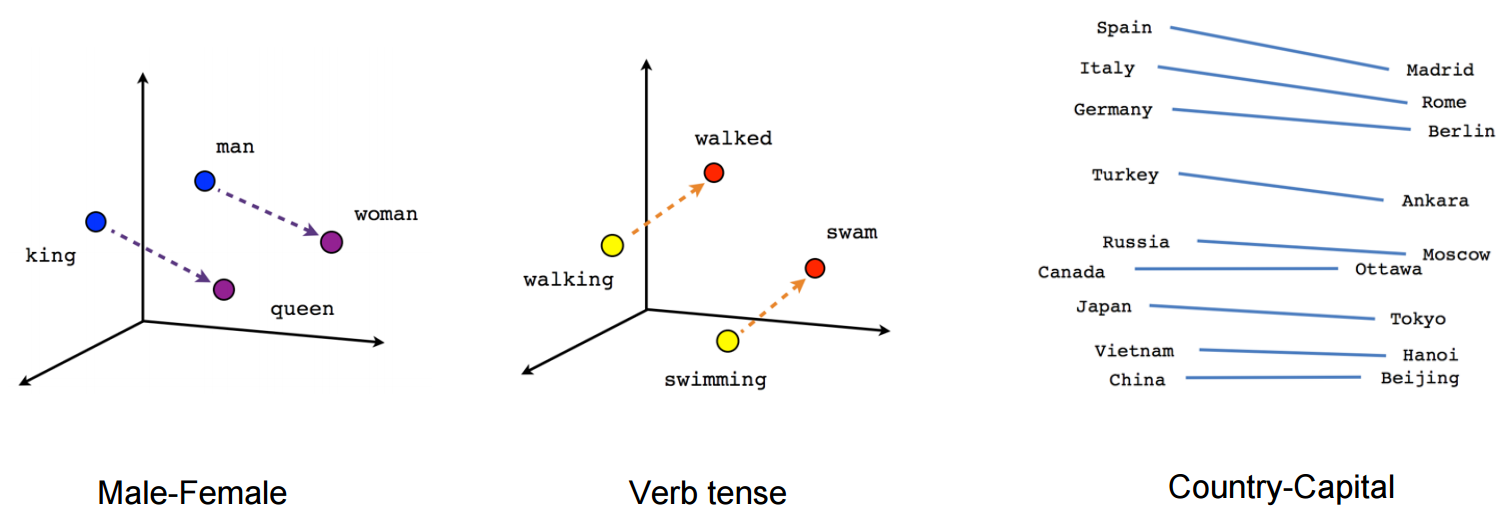
\includegraphics[scale=0.17]{pics/embeddings.png}
\end{figure}
Word embeddings can encode semantic and syntatic relationships between words.


\end{frame}




\begin{frame}{Roadmap}
\begin{scriptsize}
\begin{itemize}
\item sdfdff
\end{itemize}
\end{scriptsize}
\end{frame}



\section{Software}


\begin{frame}{AffectiveTweets}
\begin{scriptsize}

\begin{itemize}
\item Black
\end{itemize}


\end{scriptsize}
\end{frame}


\begin{frame}{WekaDeepLearning4j}
\begin{scriptsize}

\begin{itemize}
\item Black
\end{itemize}


\end{scriptsize}
\end{frame}


\begin{frame}{Wefe}
\begin{scriptsize}

\begin{itemize}
\item Black
\end{itemize}


\end{scriptsize}
\end{frame}


\begin{frame}{Ongoing Sofware Projects}
\begin{scriptsize}

\begin{itemize}
\item RiverText
\item DashAI
\end{itemize}


\end{scriptsize}
\end{frame}


\section{Shared Task}


\begin{frame}{Shared Tasks}
\begin{scriptsize}

\begin{itemize}
\item Black
\end{itemize}


\end{scriptsize}
\end{frame}


\begin{frame}
\frametitle{Questions?}
%\vspace{1.5cm}
\begin{center}\LARGE Thanks for your Attention!\\ \end{center}



\end{frame}

\begin{frame}[allowframebreaks]\scriptsize
\frametitle{References}
\bibliography{bio}
\bibliographystyle{apalike}
%\bibliographystyle{flexbib}
\end{frame}  


%%%%%%%%%%%%%%%%%%%%%%%%%%%

\end{document}
